\chapter{Theoretical Foundation}
\label{ch:theory}
This chapter introduces the Standard Model of particle physics. It also discusses
the properties of the quark level transition $b \to s \, \mu^+ \, \mu^-$, which is the main mechanism for the rare decay 
$\Lambda_b^0 \to \Lambda^0 \, \mu^+ \, \mu^-$ studied in this thesis.


\section{The Standard Model of Particle Physics}
\label{sec:standard-model}
The SM \cite{salam1959,glashow1959,weinberg1967} is the theoretical framework that describes all currently known elementary particles and their interactions, except for gravitation. At present, it provides the most accurate description of the universe at the smallest scales. However, it does not yet account for several observed phenomena, such as the presence of dark matter \cite{rubin1970}. Therefore, the predictions of the SM need to be tested against experimental data in order to measure the free parameters of the SM and to search for NP.

\subsection{Elementary Particles}
\label{subsec:fundamental-particles}
The SM classifies all known elementary particles into bosons and fermions. Fermions are half-integer spin
particles that make up matter, while bosons are integer-spin particles that mediate forces between fermions, 
with the exception of the Higgs boson. 

Fermions are further divided into quarks and leptons, each having spin $\tfrac{1}{2}$. There are three 
generations of leptons, each containing a charged lepton with charge $-\,e$, quantified by the elementary 
charge $e$, and a corresponding massless and neutral neutrino:
\begin{align*}
    \begin{array}{c}
        \begin{pmatrix}
            e \\
            \nu_e 
        \end{pmatrix},\quad
        \begin{pmatrix}
            \mu \\
            \nu_\mu
        \end{pmatrix},\quad
        \begin{pmatrix}
            \tau \\
            \nu_\tau
        \end{pmatrix}
    \end{array}
    .
\end{align*}


The charged leptons consist of the electron ($e$), muon ($\mu$), and tau ($\tau$), along with their corresponding neutrinos
($\nu_e$), ($\nu_\mu$), and ($\nu_\tau$). The three generations differ only in lepton flavor and mass, with the mass increasing
from the electron to the tau. Among them, the electron is the only stable charged lepton, while the muon and tau are
unstable and decay into lighter particles. In contrast, neutrinos are considered massless in the SM, but recent experiments have shown that they have a
small but non-zero mass, which is not accounted for in the SM \cite{neutrino_osc}. The lepton flavor, on the other hand, is an additive quantum number that distinguishes the different lepton generations. All elementary particles, including leptons, have corresponding antiparticles, which share the same mass but have opposite additive quantum numbers, such as electric charge. For example, the antiparticle of the electron is the positron ($e^+$), 
which has a charge of $+\,e$.

Quarks are also divided into three generations, consisting of an up-type quark with charge $+\tfrac{2}{3}\,e$ and a 
down-type quark with charge $-\tfrac{1}{3}\,e$:

\begin{align*}
    \begin{array}{c}
        \begin{pmatrix}
            u \\
            d
        \end{pmatrix},\quad
        \begin{pmatrix}
            c \\
            s
        \end{pmatrix},\quad
        \begin{pmatrix}
            t \\
            b
        \end{pmatrix}
    \end{array}
    .
\end{align*}

The up-type quarks are the up ($u$), charm ($c$), and top ($t$) quarks, while the corresponding
down-type quarks are the down ($d$), strange ($s$), and beauty ($b$) quarks. Analogous to leptons, 
quark generations only differ in quark flavor and mass. The mass increases from the up to the top quark
and from the down to the beauty quark, respectively. Since the first generation of quarks consists of the 
lightest up-type and down-type quarks, it is the only one that is stable.
Quarks also carry a property called color charge, which is related to the strong
force. The color charge can be red ($r$), green ($g$), or blue ($b$), and
also has corresponding anticolors ($\overline{r}$), ($\overline{g}$), and ($\overline{b}$).
Only color-neutral states can exist, which is why quarks are never found in isolation but always bound in so-called hadrons.
This phenomenon is called confinement and is caused by the linearly increasing potential of the strong force between
quarks. Hadrons are classified into baryons and mesons. Baryons are composed of three quarks,
whereas mesons consist of a quark paired with an antiquark. Recent experiments have shown that four- and five-quark states
exist as well, which are called tetraquarks and pentaquarks, respectively \cite{tetraquarks, pentaquarks}. 
% Only the first generation of fermions is stable, therefore all stable particles are composed only of up and down quarks and electrons.

Bosons, on the other hand, are divided into gauge bosons with spin $1$ and the scalar boson with spin $0$. 
The gauge bosons are responsible for mediating three fundamental forces between fermions. These three fundamental
forces are the electromagnetic, weak, and strong forces. The photon ($\gamma$) is the force carrier
of the electromagnetic interaction and couples to electrically charged particles. It is massless and electrically neutral.
The strong interaction is mediated by gluons ($g$), which are massless and electrically neutral. However, unlike photons,
they possess color charge and interact exclusively with quarks, which also carry color charge. There are eight types of gluons,
corresponding to combinations of the three color charges and their respective anticolors. Lastly, the mediators of the weak
interaction are the $W$ and $Z$ bosons. The $W$ bosons come in two charged forms, $W^+$ and $W^-$, both of which have mass.
They interact only with left-handed particles and right-handed antiparticles that carry weak isospin. 
The $Z$ boson, on the other hand, carries mass as well but is electrically neutral. It couples to both left- and right-handed particles
and antiparticles, with a coupling that depends on weak isospin and electric charge. 
%The interactions between particles via bosons are crucial to the formation and decay of particles. They enable the existence of larger structures such as atoms and molecules as well.

In the SM, the Higgs boson \cite{atlas2012, cms2012}, denoted by $H$, is the only scalar boson. It is electrically neutral, has zero spin, and carries mass. The Higgs boson is an excitation of the Higgs field, through which elementary particles acquire mass via the Yukawa coupling.

\subsection{CKM Matrix}
\label{sec:ckm-matrix}
The quark flavor is not conserved in the weak interaction. This means that quarks can change their flavor
through the exchange of $W$ bosons. The Cabibbo--Kobayashi--Maskawa (CKM) matrix \cite{cabibbo1963, kobayashi1973}
\begin{align*}
    V_{\text{CKM}} = \begin{pmatrix}
        V_{ud} & V_{us} & V_{ub} \\
        V_{cd} & V_{cs} & V_{cb} \\
        V_{td} & V_{ts} & V_{tb}
    \end{pmatrix}
\end{align*}
quantifies the mixing of quark flavors in the weak interaction. It is a unitary matrix that describes how quark mass
eigenstates are transformed into the eigenstates that participate in the weak interaction. Each element of the CKM matrix
is a complex number that represents the coupling of two quark flavors and defines the probability of each flavor-changing
transition. The values of the CKM matrix are not predicted by the SM, but can be determined through experimental measurements.
The most recent absolute values of the CKM matrix elements \cite{pdg2024} are 
\begin{align*}
    \vert V_{\text{CKM}} \vert = \begin{pmatrix}
        0.97435  & 0.22501 & 0.003732 \\
        0.22487  & 0.97349 & 0.04183 \\
        0.00858  & 0.04111 & 0.999118
    \end{pmatrix}.
\end{align*} 
It is worth noting that the CKM matrix is not diagonal and has a hierarchical structure, meaning that cross-generation transitions are possible but suppressed. 

A Flavor-Changing Neutral Current (FCNC) describes a transition where a quark changes its flavor without
changing its electric charge. Since flavor changes are mediated by $W$ bosons, only transitions between up-type and down-type
quarks are allowed. Therefore, FCNCs are not possible at tree-level in the SM, as the charge changes between up-type and 
down-type quarks. However, they can occur at higher orders through loop diagrams, which are suppressed due to the high
number of vertices.


\section{\texorpdfstring{The Decay $\Lambda_{\text{b}}^0 \to \Lambda^0 \, \mu^+ \, \mu^-$}{The Decay Lambda_b to Lambda mumu}}
\label{sec:decay-lambda-b}
As discussed in \cref{sec:standard-model}, the SM needs to be tested against experimental data in order to search for NP.
One way to do this is to study rare decays, which are processes that are highly suppressed in the SM and therefore sensitive to the smallest deviations 
from its predictions. This thesis investigates the rare baryonic decay $\Lambda_{\text{b}}^0 \to \Lambda^0 \, \mu^+ \, \mu^-$. It allows the study of the
FCNC transition $b \to s \, \mu^+ \, \mu^-$, which is the quark level transition that happens in the rare decay on a hadronic level due to confinement.
The two main processes for $b \to s \, \mu^+ \, \mu^-$ transitions are the penguin and $W$ boson box diagrams, which are 
shown in \cref{fig:decay-channels}.
\begin{figure}
    \centering
    \begin{subfigure}[b]{0.45\textwidth}
        \centering
        \tikzfeynmanset{compat=1.1.0}
        \begin{tikzpicture}
            \begin{feynman}
                \vertex (ib) {$b$};
                \vertex[right=2cm of ib] (a);
                \vertex[right=2cm of a] (b);
                \vertex[right=1cm of a] (h);
                \vertex[above=1.2cm of h] (c);
                \vertex[above right=1cm and 1.5cm of c] (d);
                \vertex[above right=1cm and 1.5cm of d] (e) {$\mu^-$};
                \vertex[below right=1cm and 1.5cmof d] (f) {$\mu^+$};
                \vertex[right=2cm of b] (fs) {$s$};
                
                \diagram* {
                    (ib) -- [fermion] (a) -- [boson, edge label=$W^-$] (b) -- [fermion] (fs),
                    (a) -- [fermion, half left, looseness=2] (b),
                    (c) -- [boson, edge label=$\gamma$/$Z$] (d),
                    (d) -- [fermion] (e),
                    (d) -- [anti fermion] (f),

                };
            \end{feynman}
        \end{tikzpicture}
        \caption{Penguin.}
        \label{fig:penguin-diagram}
    \end{subfigure}
    \hfill
    \begin{subfigure}[b]{0.45\textwidth}
        \centering
        \tikzfeynmanset{compat=1.1.0}
        \begin{tikzpicture}
            \begin{feynman}
                \vertex (ib) {$b$};
                \vertex[right=2cm of ib] (a);
                \vertex[right=2cm of a] (b);
                \vertex[right=2cm of b] (fs) {$s$};
                \vertex[above right=1.5cm and 0.5cm of a] (c);
                \vertex[above right=1.5cm and 0.5cm of b] (d);
                \vertex[above right=1.5cm and 0.5cm of c] (e) {$\mu^+$};
                \vertex[above right=1.5cm and 0.5cm of d] (f) {$\mu^-$};
                
                \diagram* {
                (ib) -- [fermion] (a) -- [fermion] (b) -- [fermion] (fs),
                (a) -- [boson, edge label=$W^-$] (c),
                (b) -- [boson, edge label=$W^+$] (d),
                (c) -- [fermion] (d),
                (c) -- [anti fermion] (e),
                (d) -- [fermion] (f),

                };
            \end{feynman}
        \end{tikzpicture}
        \caption{$W$ boson box.}
        \label{fig:w-box-diagram}
    \end{subfigure}
    \caption{The decay $b \to s \, \mu^+ \, \mu^-$. The decay can occur over two channels: the penguin (left) and $W$ boson box (right) diagrams.}
    \label{fig:decay-channels}
\end{figure}

Measurements of mesonic and baryonic decays involving the $b \to s \, \ell^+ \, \ell^-$ transition have shown deviations in various observables such as differential branching fractions and angular observables \cite{b-anomalies_1, b-anomalies_2}. They show a consistent pattern across multiple decays and observables, and are therefore referred to as $B$-anomalies. These anomalies are a hint for NP and need further investigation. This is particularly true in the baryonic sector of $b$-hadrons, as they can offer complementary insights to the mesonic decays that have already been studied extensively.

\subsection{\texorpdfstring{The $q^2$ spectrum of the transition $b \to s \, \ell^+ \, \ell^-$}{The q2 spectrum of the transition b to s mumu}}
\label{sec:q2-spectrum}
\cref{fig:q2-spectrum} shows the $q^2$ spectrum of the transition $b \to s \, \ell^+ \, \ell^-$, with $q^2$ being the invariant mass squared 
of the lepton pair, which quantifies the amount of energy transferred from the hadronic system to the leptons. The $q^2$ spectrum is an important 
observable, as it is sensitive to the underlying physics of the transition.
\begin{figure}
    \centering
    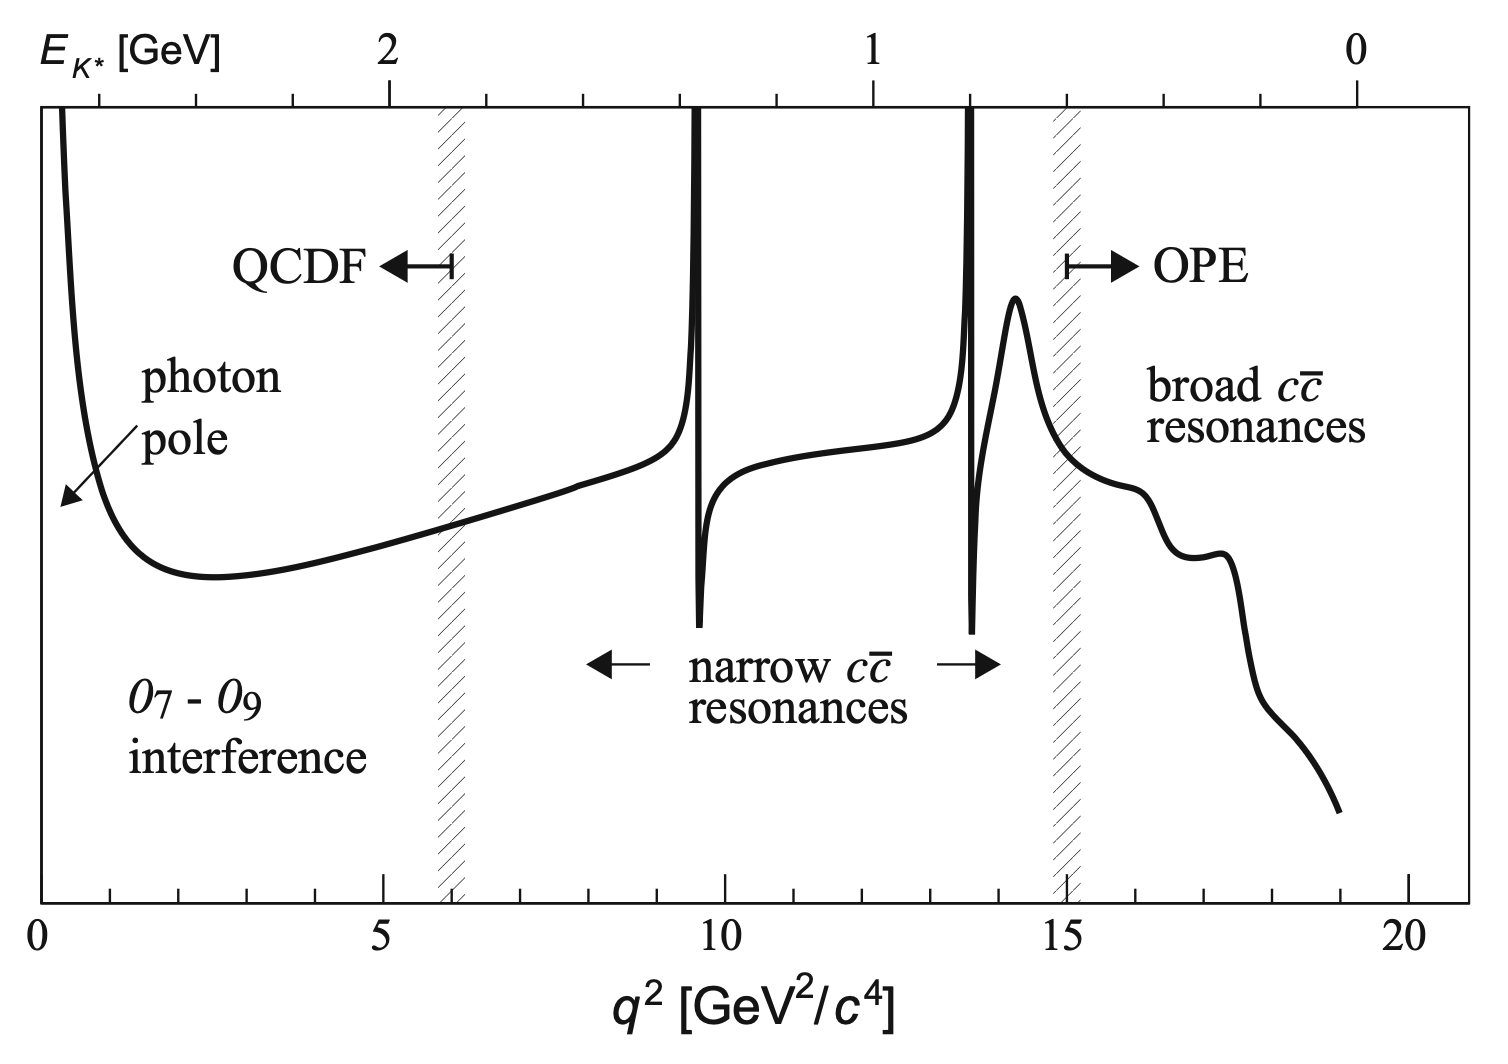
\includegraphics[width=0.9\textwidth]{figures/q2.png}
    \caption{A typical $q^2$ spectrum of the transition $b \to s \, l^+ \, l^-$, taken from \cite{blake2015}.}
    \label{fig:q2-spectrum}
\end{figure}

For low $q^2$, the spectrum is dominated by the photon pole originating from the decay $b \to s \, \gamma$, where the $\gamma$
further decays into a lepton pair. The central region is characterized by the narrow charmonium resonances $J/\psi$ and $\psi(2S)$,
each of which decays into a lepton pair. In the high $q^2$ region, above $\qty{15}{\giga\electronvolt\squared\per\lightspeed\tothe{4}}$,
the spectrum is dominated by the already mentioned penguin and $W$ boson box diagrams.